\section{Clusters}

Clusters are regarded as a subset of distributed systems. Unlike distributed systems the nodes in a cluster are mostly homogeneous having the same hardware and operating system. They are dedicated to performing tasks that are well defined by acting as one single entity. The brief explanation of clusters may sound similar to distributed systems and hence to distinguish between the two classes the table \ref{table:cluster_vs_distributed_systems} lists some of the key differences between clusters and distributed systems.

\begin{table}[h]
  \centering
  \caption{Clusters vs. Distributed systems}
  \label{table:cluster_vs_distributed_systems}
  \begin{tabular}{ccc}
    \toprule
    Aspect & Clusters & Distributed systems\\
    \midrule
    Structure & Homogeneous & Heterogeneous\\
    Scale & Small scale & Medium or large scale\\
    Task & Specialized & General\\
    Security & Nodes trust each other & Nodes do not trust each other\\
    \bottomrule
  \end{tabular}
\end{table}

\subsection{Cluster Attributes}

Clusters can be used for various tasks ranging from general purpose tasks to resource intensive scientific computations. The two important attributes of clusters are load balancing and high availability.

\begin{itemize}
  \item \textbf{Load-balancing:} This refers to the balancing load of computation among different nodes of the cluster. The balancing technique can range from simple round-robin fashion to any sophisticated algorithms depending on the nature of the task that needs to be performed. Figure \ref{figures:cluster1} depicts a cluster setup in which a dispatcher sends the web requests to the servers ensuring that the load is evenly distributed among them.
  
    \makeatletter
    \setlength{\intextsep}{25pt}
    \makeatother

    \begin{figure}[h!]
    \centering
    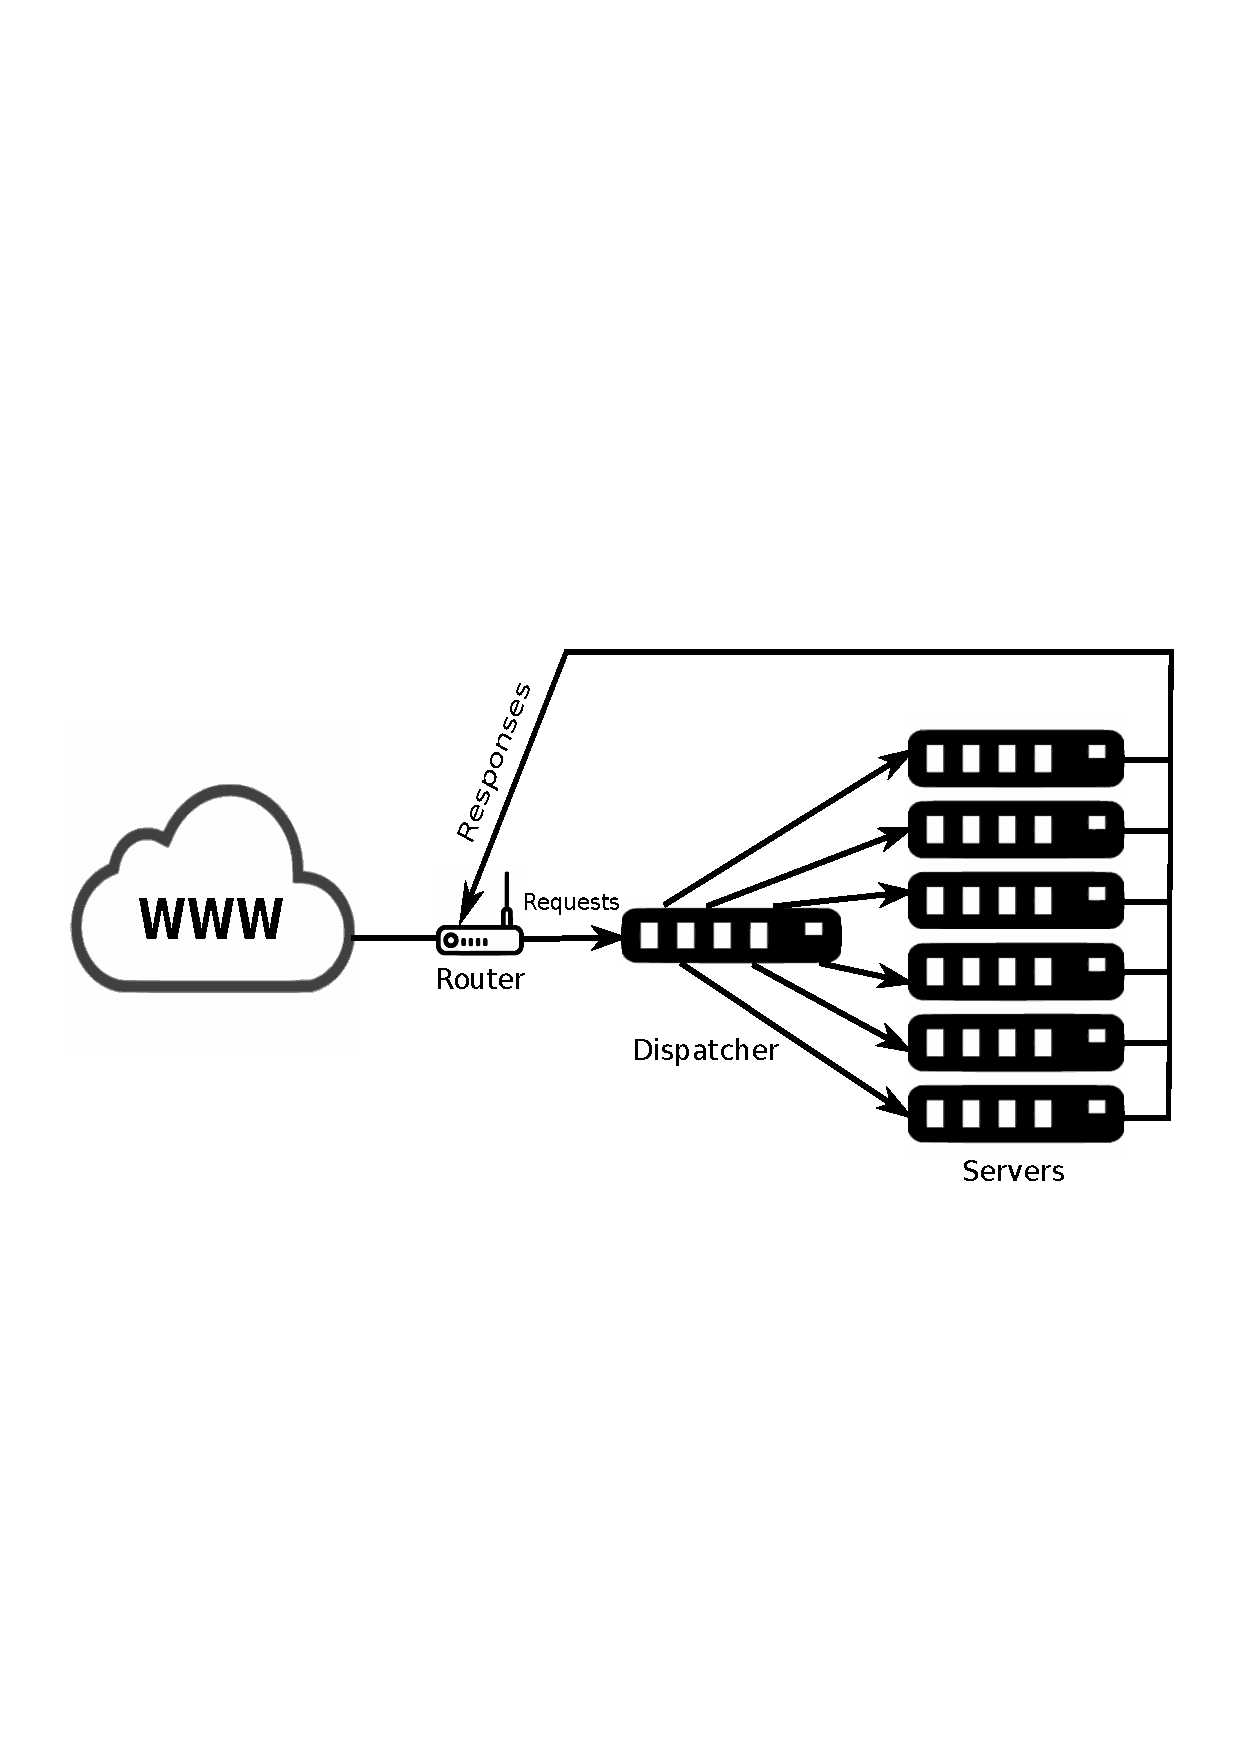
\includegraphics[keepaspectratio, width=.7\textwidth, trim={0 8cm 0 9cm},clip]{cluster1.pdf}
    \caption{Load-balancing cluster Example}\label{figures:cluster1}
    \end{figure}

  \item \textbf{High-availability:} This refers to providing fault tolerance eliminating the single point of failure. This is done by having redundant nodes which take over the nodes that fail during the regular operation. They are also referred as failover clusters. Figure \ref{figures:cluster} depicts a file service cluster setup where the active machine serves files to the clients and the standby machine acts as a backup. The backup keeps its copy of files updated concerning the active machine. In case the active machine fails, the backup machines realizes this and takes over the active server and continues to serve the files to the clients. Thus even in a case of failure, the service is not shutdown completely.

    \makeatletter
    \setlength{\intextsep}{25pt}
    \makeatother

    \begin{figure}[h!]
    \centering
    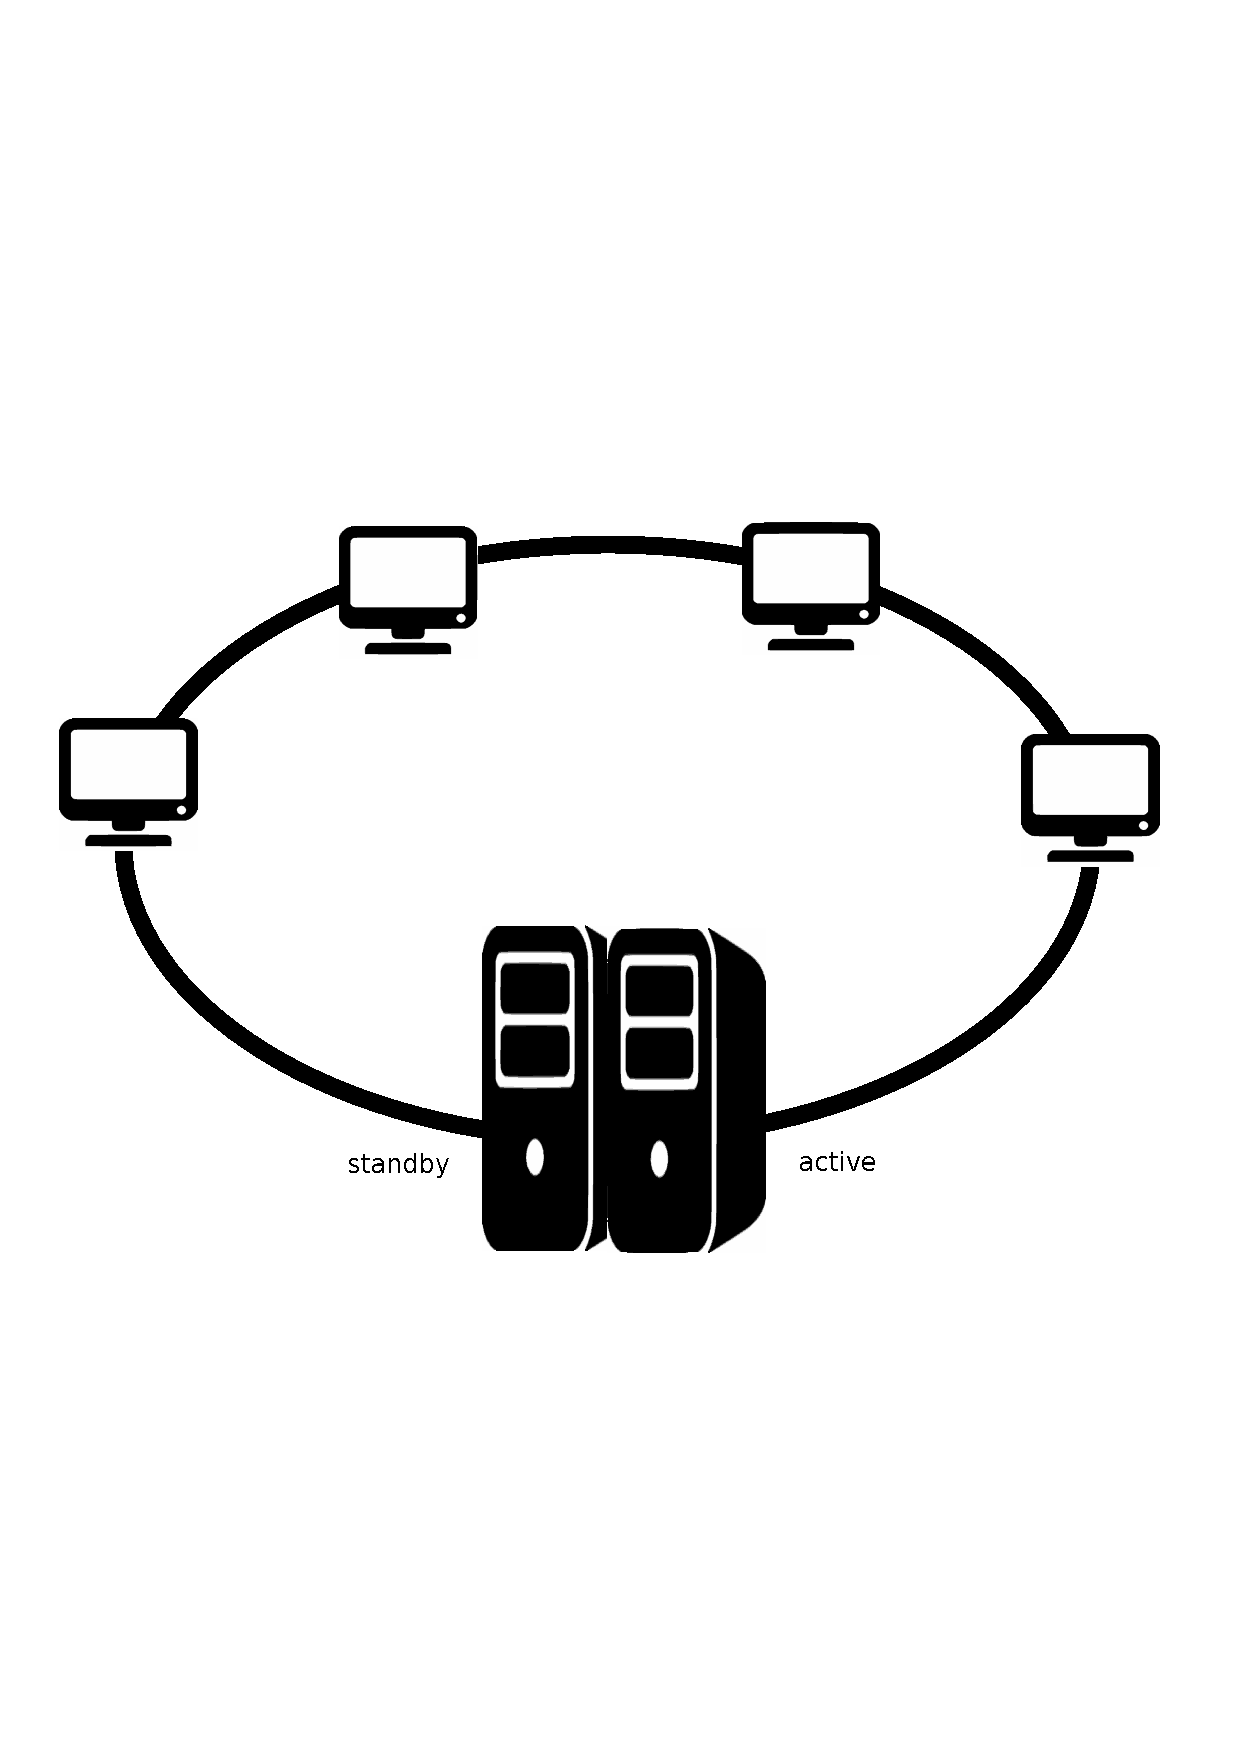
\includegraphics[keepaspectratio, width=.7\textwidth, trim={0 8cm 0 7cm},clip]{cluster.pdf}
    \caption{High-availability cluster Example}\label{figures:cluster}
    \end{figure}

\end{itemize} 

